\chapter{Results}


Describe the initial conditions, table, cool


\section{BEM alligned rotor \textcolor{red}{BERNAT}}


\subsection{Main outputs \textcolor{red}{BERNAT}}


\subsubsection{Angle of attack and inflow angle \textcolor{red}{BERNAT}}

\subsubsection{Axial and azimuthal inductions \textcolor{red}{BERNAT}}

\subsubsection{Thrust and azimuthal loading \textcolor{red}{BERNAT}}

\subsubsection{Total thrust and torque \textcolor{red}{BERNAT}}


\section{BEM yawed rotor \textcolor{blue}{NIKLAS}}


\subsection{Main outputs \textcolor{blue}{NIKLAS}}


\subsubsection{Angle of attack and inflow angle \textcolor{blue}{NIKLAS}}

\subsubsection{Axial and azimuthal inductions \textcolor{blue}{NIKLAS}}

\subsubsection{Thrust and azimuthal loading \textcolor{blue}{NIKLAS}}

\subsubsection{Total thrust and torque \textcolor{blue}{NIKLAS}}

\section{Influence of the tip correction \textcolor{green}{CARLOS}}

The results shown in this section were obtained for the rotor described in the assignment instructions, operating with a tip speed ratio $ \lambda = 8 $ and no yaw. It can be seen that the tip correction reduces the power and thrust, resulting in a worse performance. Indeed, the rotor without the tip correction has a higher $ C_P/C_T $ ratio.

Near the blade tip, the flow angle $ \phi $ is reduced due to the tip vortex (Figure \ref{img:tc-phi}), because it induces a larger axial velocity (Figure \ref{img:tc-a}). Having a lower flow angle $ \phi $ results in a reduced power extraction, which is proportional to $ c_l \sin \phi - c_d \cos \phi $ (Figure \ref{img:tc-dcp-dmu}) \cite{weh-ch3}. However, reducing the flow angle $ \phi $ contributes to an increase of the thrust, since it is proportional to $ c_l \cos \phi + c_d \sin \phi $.

Note that $ c_l $ also decreases due to the reduction of $ \phi $, because it implies a decrease of the angle of attack $ \alpha $ (Figure \ref{img:tc-alpha}). Moreover, the relative velocity, which also affects the loads, will also be larger for the case without tip correction.

The tip correction tries to account for this effect. The expression Prandtl derived for that factor is shown in equation \ref{eq:f-prandtl}. Its value over the blade is plotted in Figure \ref{img:tc-f}. It relates the induction factor near the blade $ a_b $ with the azimuth average $ a $: $ a_b = a/f $ \cite{weh-ch3}.

\begin{equation}
f(\mu) = \frac{2}{\pi} \arccos \left[ \exp \left( - \frac{B}{2} \left( \frac{1-\mu}{\mu} \right) \sqrt{1+\frac{\lambda^2\mu^2}{(1-a)^2}} \right) \right]
\label{eq:f-prandtl}
\end{equation}

\begin{itemize}
	
	\item Power coefficient $ C_P $
	\begin{itemize}
		\item Tip correction: 0.4528
		\item No tip correction: 0.4757
		\item Increase: 5.05 \%
	\end{itemize}
	
	\item Thrust coefficient $ C_T $
	\begin{itemize}
		\item Tip correction: 0.6581
		\item No tip correction: 0.6691
		\item Increase: 1.67 \%
	\end{itemize}
	
	\item Power to thrust ratio $ C_P/C_T $
	\begin{itemize}
		\item Tip correction: 0.6880
		\item No tip correction: 0.7109
		\item Increase: 3.32 \%
	\end{itemize}
	
\end{itemize}

\begin{figure}[htbp]
	\centering
	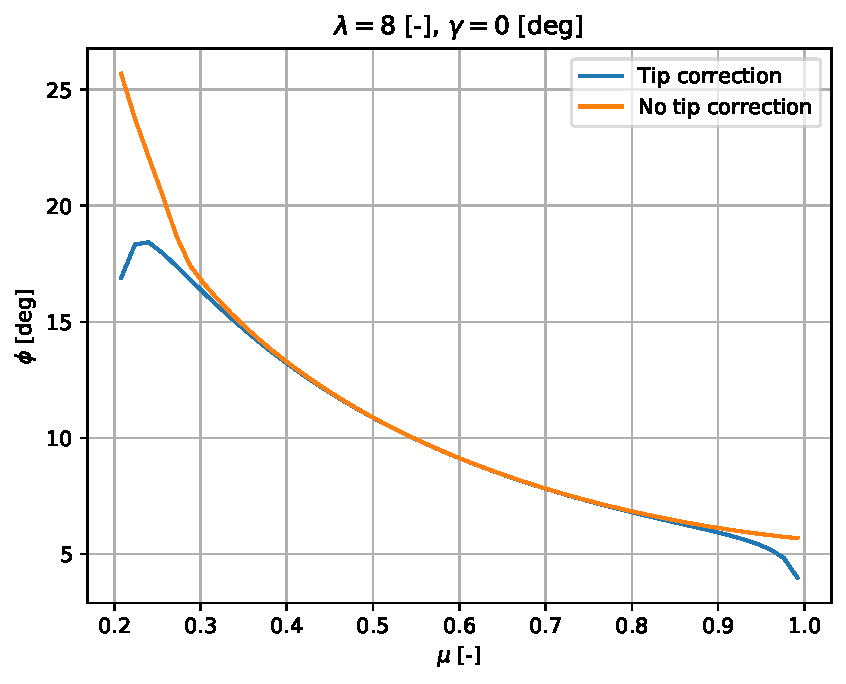
\includegraphics[height=0.45\textheight]{./img/tip-correction/phi.pdf}
	\caption{Flow angle distribution with and without tip correction.}
	\label{img:tc-phi}
\end{figure}

\begin{figure}[htbp]
	\centering
	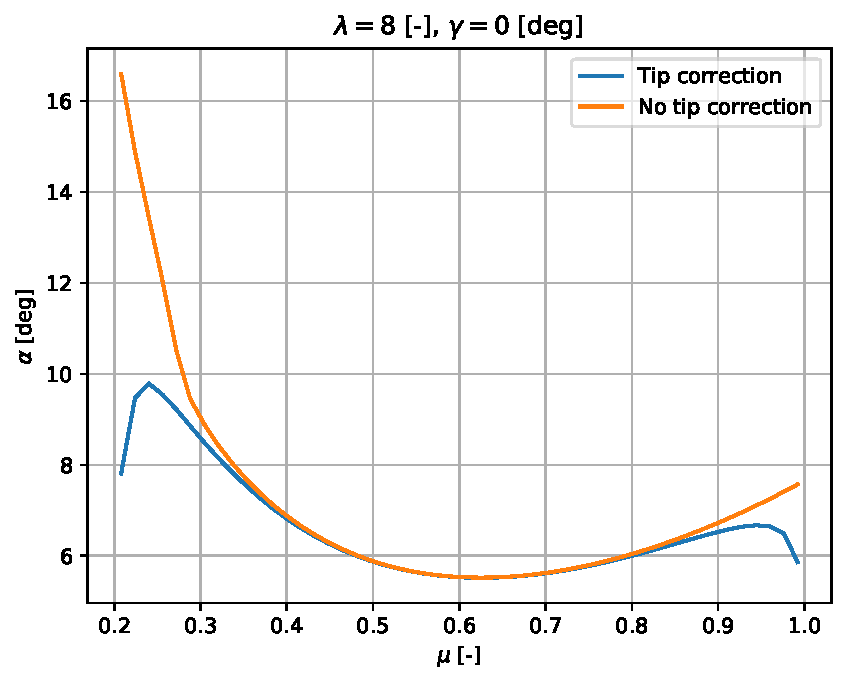
\includegraphics[height=0.45\textheight]{./img/tip-correction/alpha.pdf}
	\caption{Angle of attack distribution with and without tip correction.}
	\label{img:tc-alpha}
\end{figure}

\begin{figure}[htbp]
	\centering
	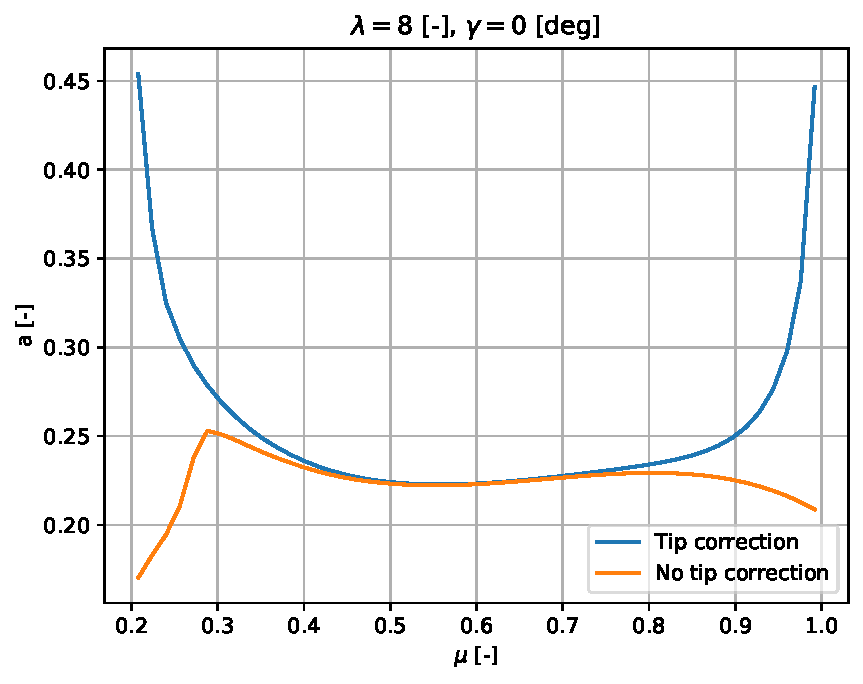
\includegraphics[height=0.45\textheight]{./img/tip-correction/a.pdf}
	\caption{Axial induction distribution with and without tip correction.}
	\label{img:tc-a}
\end{figure}

\begin{figure}[htbp]
	\centering
	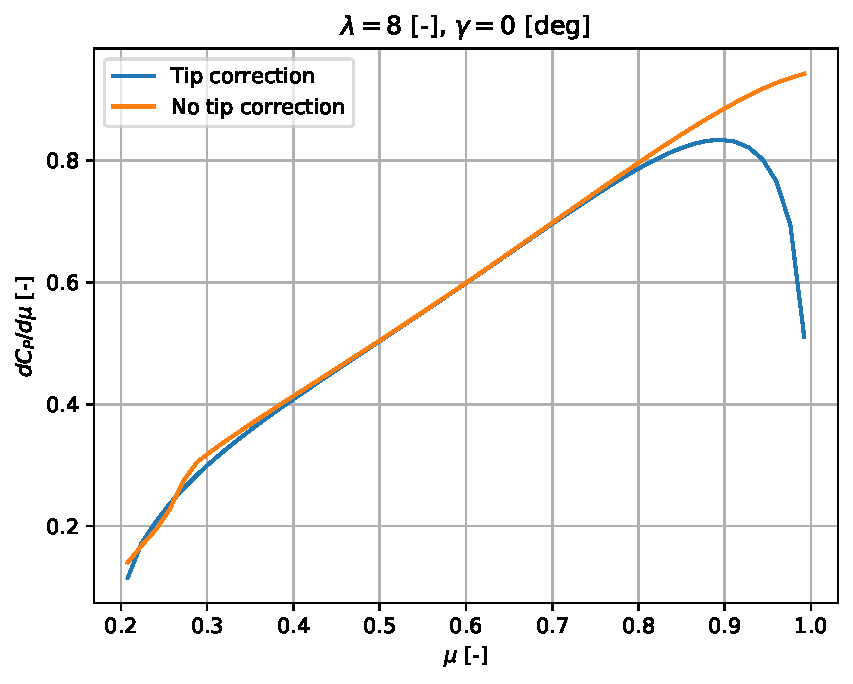
\includegraphics[height=0.45\textheight]{./img/tip-correction/dcp_dmu.pdf}
	\caption{Power coefficient distribution with and without tip correction.}
	\label{img:tc-dcp-dmu}
\end{figure}

\begin{figure}[htbp]
	\centering
	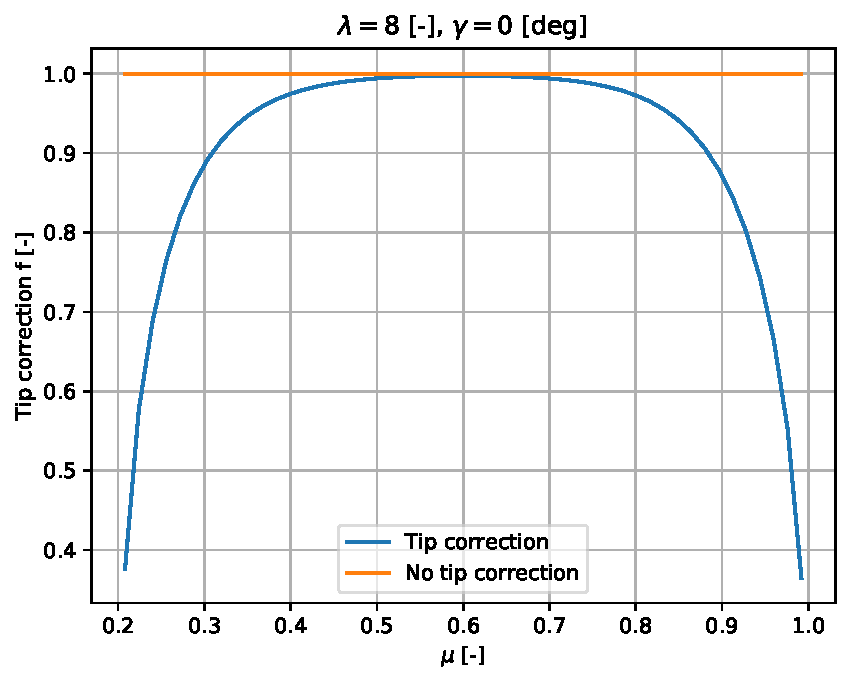
\includegraphics[height=0.45\textheight]{./img/tip-correction/f.pdf}
	\caption{Prandtl's tip loss factor distribution with and without tip correction.}
	\label{img:tc-f}
\end{figure}

\section{Influence of numerical discretization \textcolor{red}{BERNAT}}

\section{Evaluation of stagnation enthalpy \textcolor{green}{CARLOS}}

If heat exchange, viscous forces and compressibility effects are neglected, the flow temperature does not change. Therefore, it can be assumed that the air's internal energy is always constant. Then, the changes in stagnation enthalpy and stagnation pressure are equivalent. The mechanical energy equation (\ref{eq:mech-energy}) describes how the stagnation pressure $ p_t $ changes. Note that it has been obtained as the scalar product of the momentum equation and the velocity vector.

\begin{equation}
	\vec{v} \cdot \vec{\nabla} p_t = \vec{v} \cdot \vec{\nabla} \cdot \vec{\vec{\tau}} + \vec{v} \cdot \vec{f}
	\label{eq:mech-energy}
\end{equation}

If viscous forces are not considered, $ \tau = 0 $, the stagnation pressure can only due to the body forces $ b $ work. The only domain region where these forces are not null, and therefore, exert some work is the rotor plane. This means that the stagnation pressure only changes across the rotor plane. See equations (\ref{eq:pt-up}) and (\ref{eq:pt-down}) for the stagnation pressure expressions up and down-stream of the rotor plane respectively. They are plotted in Figure \ref{img:pt}.

\begin{equation}
	p_{t_u} = p_a + \frac{1}{2} \rho u_{\infty}^2
	\label{eq:pt-up}
\end{equation}

\begin{equation}
	p_{t_d} = p_a + \frac{1}{2} \rho u_{\infty}^2 (1-2a)^2
	\label{eq:pt-down}
\end{equation}

\begin{figure}[htbp]
	\centering
	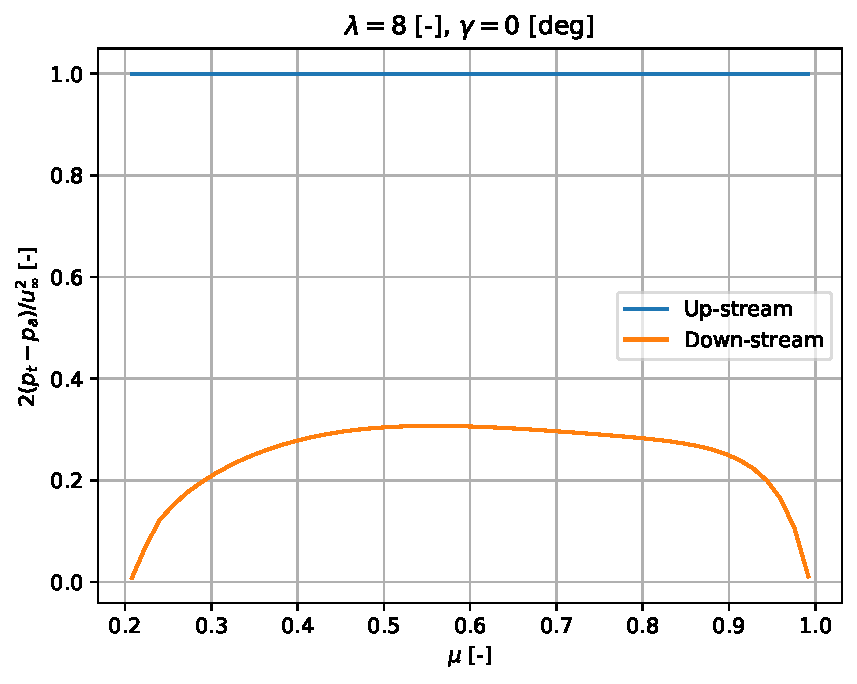
\includegraphics[height=0.45\textheight]{./img/stagnation-enthalpy.pdf}
	\caption{Stagnation enthalpy distribution.}
	\label{img:pt}
\end{figure}

\section{System of circulation and vorticity \textcolor{green}{CARLOS}}

The circulation distribution over the blade is shown in Figure \ref{img:gamma_}. It has a more or less constant shape in the centre part of the blade, and vanishes quite steeply near the root and tip. This seems reasonable, since circulation is related to lift generation by the Kutta-Joukowski theorem: $ l = \rho u_{\infty} \Gamma $. In the blade extremes, lift must be zero, since there is no surface that can create it.

\begin{figure}[htbp]
	\centering
	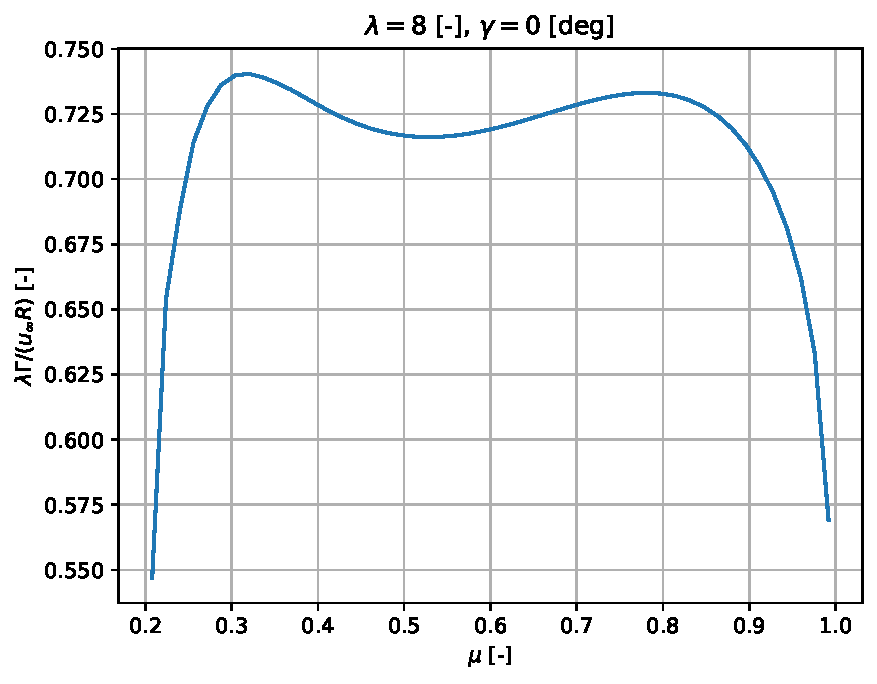
\includegraphics[height=0.45\textheight]{./img/circulation/gamma_.pdf}
	\caption{Circulation distribution.}
	\label{img:gamma_}
\end{figure}

The vorticity equation and Kutta-Jukowski theorem explain the changes observed in circulation. The thrust derivative with respect to the radius can be expressed using the Blade Element Theory, Kutta-Jukowski theorem and assuming no drag (\ref{eq:dT_dr_kj}), or using the Momentum Theory (\ref{eq:dT_dr_mt}).

\begin{equation}
	\frac{dT}{dr} = l \cos \phi = \rho w \Gamma \cos \phi
	\label{eq:dT_dr_kj}
\end{equation}

\begin{equation}
	\frac{dT}{dr} = \rho u_{\infty} (1-a) u_{\infty} 2a 2\pi r
	\label{eq:dT_dr_mt}
\end{equation}

If the expressions (\ref{eq:dT_dr_kj}) and (\ref{eq:dT_dr_mt}) are equated, it can be seen that the circulation is related to the local thrust. This is shown in Figure \ref{img:vort-forces}, where the two sides of equation (\ref{eq:gamma-ct}) are plotted. The slightly higher values for the thrust coefficient may be due to the drag contribution, which is not accounted for in the circulation.

\begin{equation}
	\frac{w \Gamma \cos \phi}{u_{\infty}^2 \pi r} = 4a(1-a) = C_T
	\label{eq:gamma-ct}
\end{equation}

\begin{figure}[htbp]
	\centering
	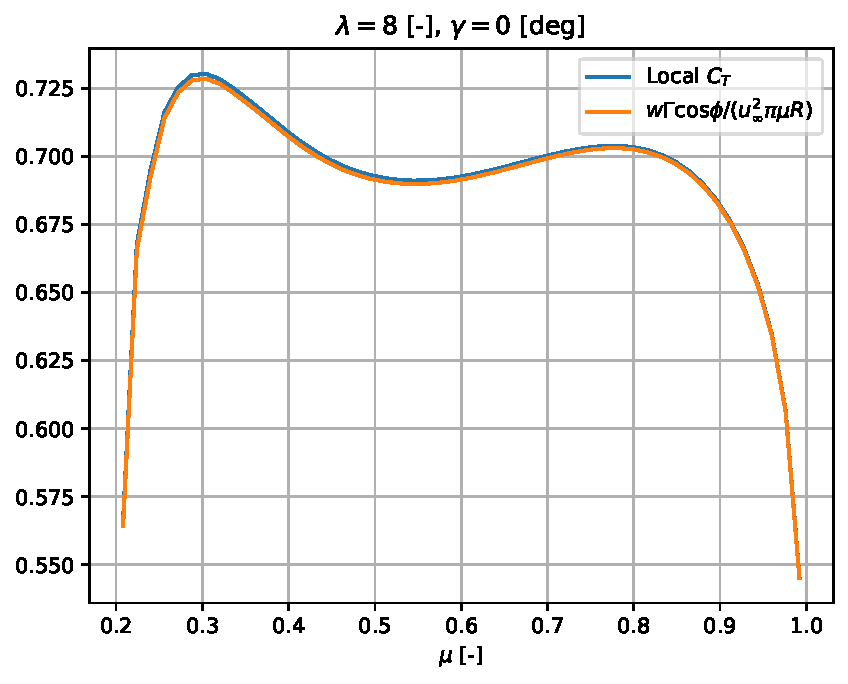
\includegraphics[height=0.45\textheight]{./img/circulation/vort-forces.pdf}
	\caption{Circulation and local thrust coefficient distribution.}
	\label{img:vort-forces}
\end{figure}

Equation (\ref{eq:gamma-ct}) is actually a different form of the vorticity equation (\ref{eq:vorticity}).

\begin{equation}
	\vec{v} \cdot \vec{\nabla} \vec{\omega} = \vec{\nabla} \times \vec{f}
	\label{eq:vorticity}
\end{equation}

Assuming there are no radial forces, and that vorticity only changes in its direction ($d\omega_i/dx_j = 0$, if $ i \neq j $), the vorticity equation in the tangential direction can be simplified to better show how it relates to expression (\ref{eq:gamma-ct}).

\begin{equation}
	w \cos \pi \frac{d\omega}{rd\theta} = - \frac{df_x}{dr}
	\label{eq:vort-tang}
\end{equation}

If equation (\ref{eq:vort-tang}) is integrated over the volume, expression \ref{eq:gamma-ct} is obtained. Remark that $ \int 1/r d\omega/d\theta dV = - \int \omega dS = - \Gamma $, and $ \int df_x/dr dV = dT/dr $.

The same procedure can be done for the vorticity generation in the axial direction. In this case, the vorticity equation is the one shown in (\ref{eq:vort-axial}). The relationship between the circulation and tangential force is given by equation (\ref{eq:gamma-cs}).

\begin{equation}
	w \sin \pi \frac{d\omega}{dx} = \frac{df_{\theta}}{dr}
	\label{eq:vort-axial}
\end{equation}

\begin{equation}
	\frac{dS}{dr} = l \sin \phi = \rho w \sin \phi \Gamma = \rho u_{\infty} (1-a) \Omega r 2a' 2 \pi r
	\label{eq:gamma-cs}
\end{equation}

The relationship between the tangential force and generation of circulation in the axial direction is depicted in Figure \ref{img:vort-forces-ax}. The differences observed may be due to the drag, which reduces the tangential force created by the lift.

\begin{figure}[htbp]
	\centering
	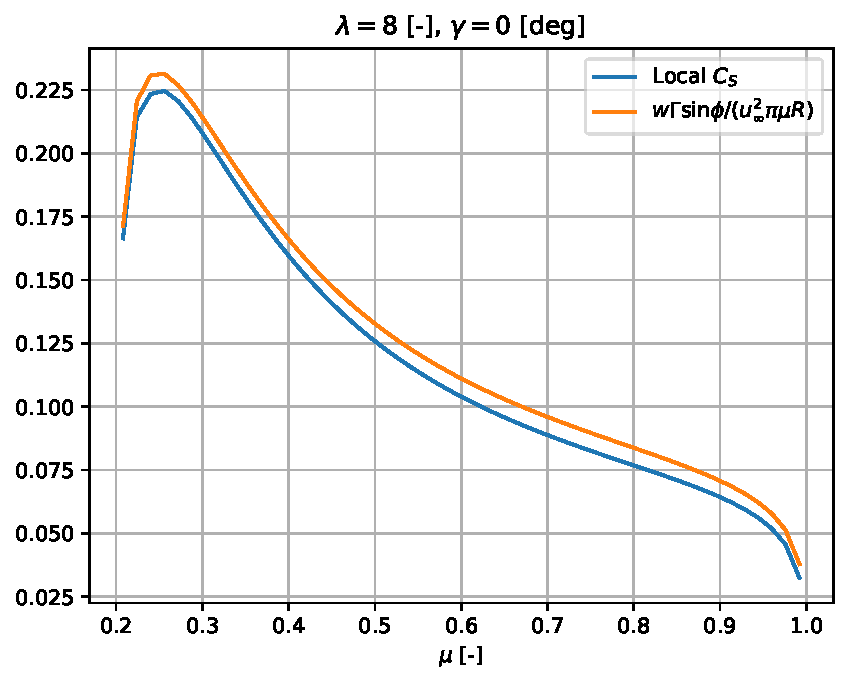
\includegraphics[height=0.45\textheight]{./img/circulation/vort-forces-ax.pdf}
	\caption{Circulation and local tangential coefficient distribution.}
	\label{img:vort-forces-ax}
\end{figure}

\section{Operational point \textcolor{blue}{NIKLAS}}
